\titlepage{
\begin{center}
{\Large\bfseries\color{\MaCouleur} Philippe \bsc{De Sousa}}

\vspace*{\stretch{1}}

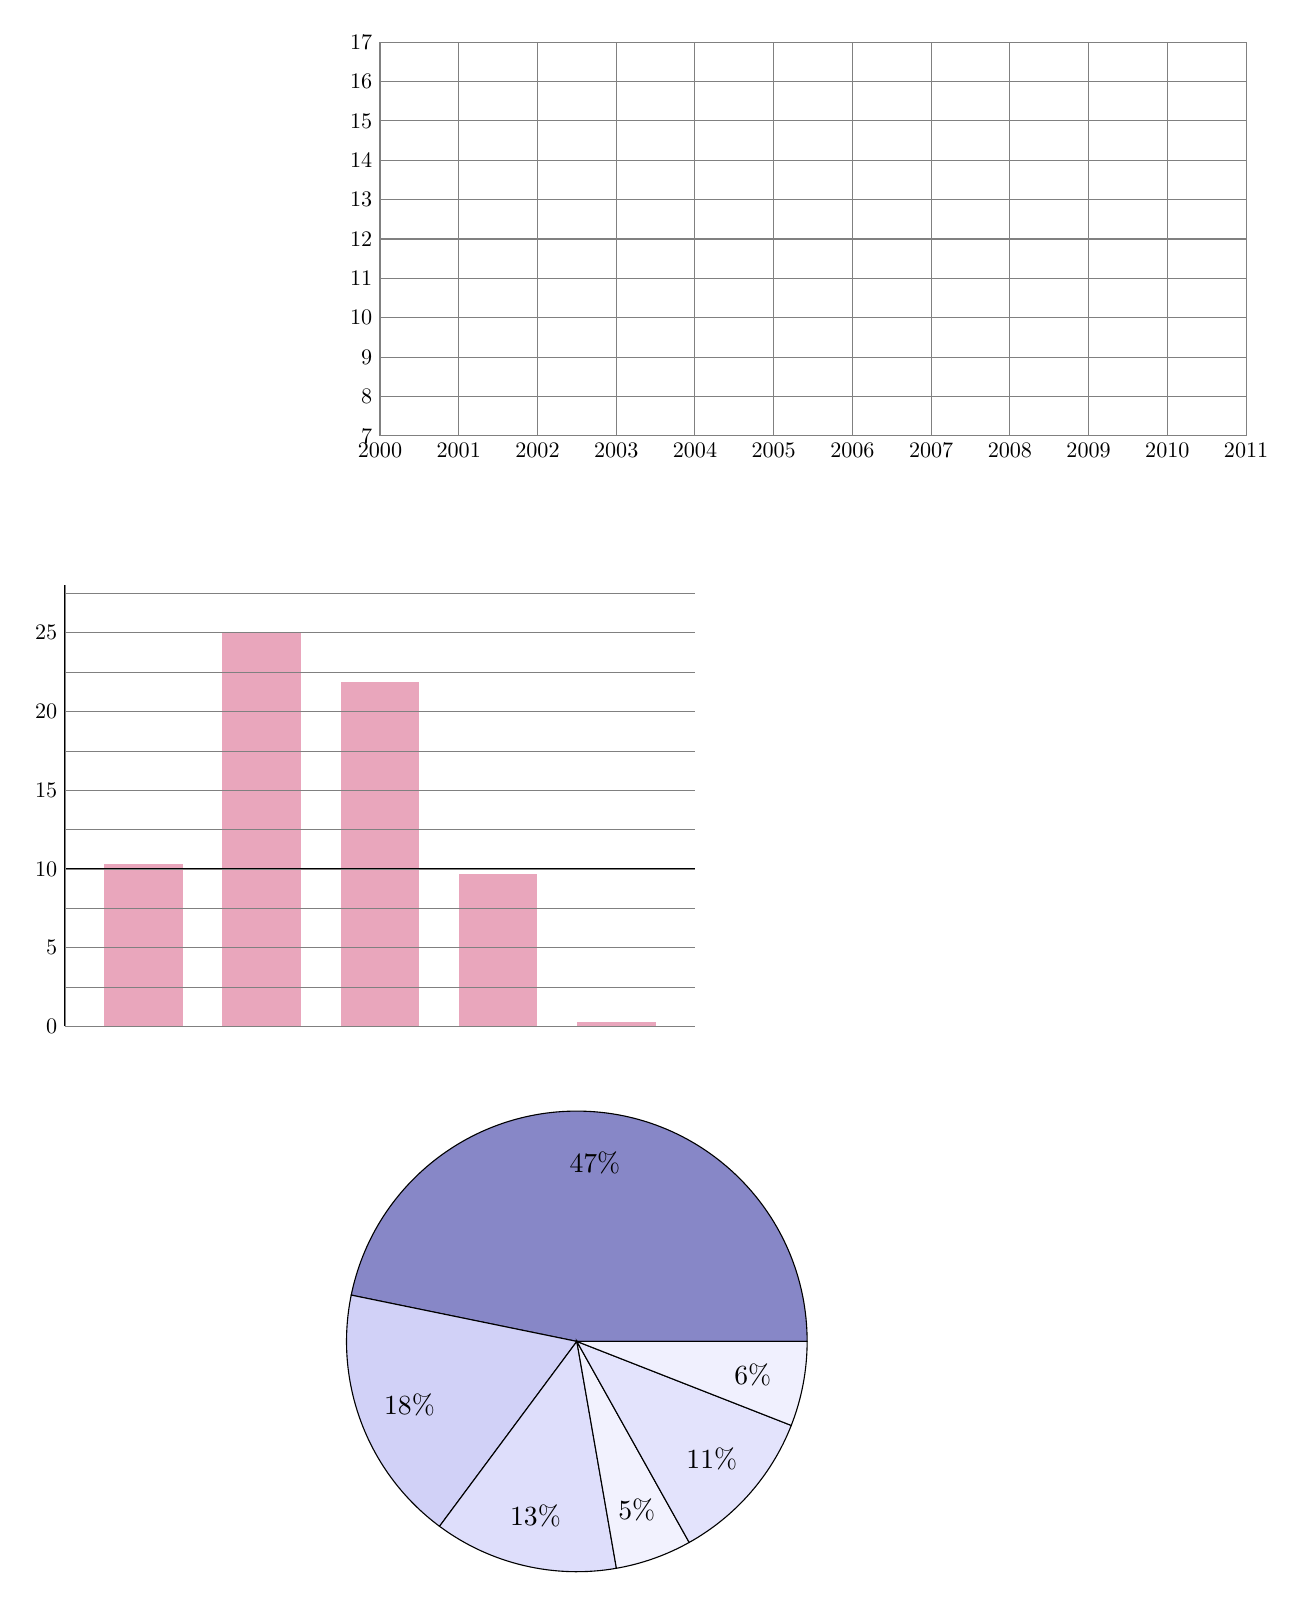
\begin{tikzpicture}
\begin{scope}[xscale=1,yscale=0.2,xshift=-1cm]
\newcommand{\Conso}{(1,10.3)(2.5,25)(4,21.9)(5.5,9.7)(7,0.3)}
\draw[line width=10mm,color=purple!35] plot[ycomb] coordinates {\Conso};
\draw (0,0) grid[xstep=9,ystep=5] (8,28);
\draw[gray,very thin] (0,0) grid[xstep=9,ystep=2.5] (8,28);
\foreach \y in {0,5,...,25} \draw (0,\y) node[left,scale=0.8]{\y};
\end{scope}

\begin{scope}[xshift=3cm,yshift=4cm,yscale=0.5]
\draw[color=OliveGreen,line width=1.5pt] plot[mark=triangle,mark size=3pt] file {Titre1.txt};
\draw[color=blue,line width=1.5pt] plot[mark=diamond,mark size=3pt] file {Titre2.txt};
\draw[thin,gray] (0,7) grid (11,17);
\foreach \y in {7,8,...,17} \draw (0,\y) node[left,scale=0.8]{\y};
\foreach \x in {2000,2001,...,2011} \draw (\x-2000,7) node [below,scale=0.8] {\x};
\end{scope}

\begin{scope}[xshift=5.5cm,yshift=-4cm,scale=0.65]
%\draw[fill=black!47!blue!47] (0,0)--(0:4.5)arc(0:168.4:4.5)--cycle;
%\draw (84:4) node {47\%};
%\draw (84:5.6) node {\bsc{tva}};
\foreach \a/\b/\p/\c in
{
0/168.4/47/\bsc{tva},
168.4/233.4/18/Revenus,
233.4/279.9/13/Sociétés,
279.9/299.2/5/\bsc{tipp},
299.2/338.6/11/{\scriptsize Recettes fiscales},
338.6/360/6/{\scriptsize Recettes}
}{
\draw[fill=black!\p!blue!\p]
(0,0) -- (\a:4.5) arc (\a:\b:4.5) -- cycle;
\draw ({(\a+\b)/2}:3.5) node {\p\%};
}
\end{scope}
\end{tikzpicture}

\begin{tikzpicture}[remember picture,overlay]
\begin{scope}
\node [rotate=45,scale=8,text opacity=0.2]
at (current page.center) {\color{\MaCouleur}\scshape Mathématiques};
\end{scope}
\begin{scope}[xshift=5.5cm,yshift=8cm]
\draw[color=\MaCouleur] (0,0) node[scale=8] {\premiere};
\draw[color=\MaCouleur] (-0.2,-0.15) node[below,scale=6] {\stmg};
\node [below=7cm,scale=4,color=\MaCouleur] at (-0.2,-0.15) {Activités};
\end{scope}
\end{tikzpicture}

\vspace*{\stretch{1}}

D'après le programme $\NP{2012}$
\end{center}
} 